\documentclass[compress, aspectratio=169]{beamer}
\usepackage[english]{babel}

\usepackage{amsthm}
\usepackage{mathtools}
\usepackage{physics}
\usepackage{calligra}
\usepackage{csquotes}
\usepackage{tensor}
\usepackage[thicklines]{cancel}
\usepackage{tcolorbox}
\usepackage{pstricks}

\usepackage{multirow}
\usepackage{multicol}
\usepackage{bigdelim}

\usepackage{tabularx}
\usepackage{tikz}
\usepackage{mathtools}
\usepackage{amsmath,amssymb}

%\usepackage[font=footnotesize,labelfont={color=orange,bf}]{caption}
\usepackage{graphicx}

\usepackage[absolute,overlay]{textpos}
%\usepackage[texcoord,grid,gridcolor=red!10,subgridcolor=green!10,gridunit=pt]{eso-pic}

\usepackage{xparse}
\NewDocumentCommand{\framecolorbox}{oommm}
    {% #1 = width (optional)
    % #2 = inner alignment (optional)
    % #3 = frame color
    % #4 = background color
    % #5 = text
    \IfValueTF{#1}
    {%
    \IfValueTF{#2}
     {\fcolorbox{#3}{#4}{\makebox[#1][#2]{#5}}}
     {\fcolorbox{#3}{#4}{\makebox[#1]{#5}}}%
    }
    {\fcolorbox{#3}{#4}{#5}}%
    }

\usepackage[natbib=true,backend=biber,style=apa, sorting=nty, citestyle=authoryear-comp]{biblatex} %Custom bibliography
    \addbibresource{bib.bib} %Load references

\AtBeginBibliography{\footnotesize}

\DeclareMathAlphabet{\mathcalligra}{T1}{calligra}{m}{n}
\DeclareFontShape{T1}{calligra}{m}{n}{<->s*[2.2]callig15}{}
\newcommand{\scriptr}{\mathcalligra{r}\,}
\newcommand{\boldscriptr}{\pmb{\mathcalligra{r}}\,}
\def\rc{\scriptr}
\def\brc{\boldscriptr}
\def\hrc{\hat\brc}
\newcommand{\ie}{\emph{i.e.}} %id est
\newcommand{\eg}{\emph{e.g.}} %exempli gratia
\newcommand{\rtd}[1]{\ensuremath{\left\lfloor #1 \right\rfloor}}
\newcommand{\dirac}[1]{\ensuremath{\delta \left( #1 \right)}}
\newcommand{\diract}[1]{\ensuremath{\delta^3 \left( #1 \right)}}
\newcommand{\e}{\ensuremath{\epsilon_0}}
\newcommand{\m}{\ensuremath{\mu_0}}
\newcommand{\V}{\ensuremath{\mathcal{V}}}
\newcommand{\prnt}[1]{\ensuremath{\left(#1\right)}} %parentheses
\newcommand{\colch}[1]{\ensuremath{\left[#1\right]}} %square brackets
\newcommand{\chave}[1]{\ensuremath{\left\{#1\right\}}}  %curly brackets

\useoutertheme{infolines}
\useinnertheme{rectangles}
\usefonttheme{professionalfonts}


\definecolor{orange}{HTML}{f28165}
\definecolor{gray}{HTML}{303030}
\definecolor{yellow}{HTML}{f0be52}
\definecolor{lightorange}{HTML}{f19e58}
\definecolor{myblue}{cmyk}{1,.72,0,.38}
\definecolor{aliceblue}{rgb}{0.94, 0.97, 1.0}

\renewcommand{\CancelColor}{\color{orange}}

\makeatletter
\newcommand{\mybox}[1]{%
  \setbox0=\hbox{#1}%
  \setlength{\@tempdima}{\dimexpr\wd0+13pt}%
  \begin{tcolorbox}[colback=orange,colframe=orange,boxrule=0.5pt,arc=4pt,
      left=6pt,right=6pt,top=6pt,bottom=6pt,boxsep=0pt,width=\@tempdima]
    \textcolor{white}{#1}
  \end{tcolorbox}
}
\makeatother

\usecolortheme[named=orange]{structure}
\usecolortheme{sidebartab}
\usecolortheme{orchid}
\usecolortheme{whale}
\setbeamercolor{alerted text}{fg=yellow}
\setbeamercolor{block title alerted}{bg=alerted text.fg!90!black}
\setbeamercolor{block title example}{bg=lightorange!60!black}
\setbeamercolor{background canvas}{bg=gray}
\setbeamercolor{normal text}{bg=gray,fg=white}
\setbeamercolor{subsection in head/foot}{bg=white, fg=gray}


\setbeamertemplate{blocks}[rectangle]
\setbeamercovered{dynamic}

\setbeamertemplate{caption}[numbered]

\setbeamertemplate{section page}
{
	\begin{centering}
		\begin{beamercolorbox}[sep=27pt,center]{part title}
			\usebeamerfont{section title}\insertsection\par
			\usebeamerfont{subsection title}\insertsubsection\par
		\end{beamercolorbox}
	\end{centering}
}

\addtobeamertemplate{navigation symbols}{}{ \hspace{1em}    \usebeamerfont{footline}%
    \insertframenumber / \inserttotalframenumber }
\setbeamertemplate{navigation symbols}{}

%\beamer@compresstrue
\defbeamertemplate*{headline}{smoothbars theme}{%
  \begin{beamercolorbox}[ht=2.125ex,dp=3.150ex]{section in head/foot}
  \insertnavigation{\paperwidth}
  \end{beamercolorbox}%

  \begin{beamercolorbox}[ht=2.125ex,dp=1.125ex,%
  leftskip=.3cm,rightskip=.3cm plus1fil]{subsection in head/foot}
  \usebeamerfont{subsection in head/foot}\insertsubsectionhead
  \end{beamercolorbox}%
}

\setbeamertemplate{subsection page}
{
	\begin{centering}
		\begin{beamercolorbox}[sep=12pt,center]{part title}
			\usebeamerfont{subsection title}\insertsubsection\par
		\end{beamercolorbox}
	\end{centering}
}

\newcommand{\hlight}[1]{\colorbox{violet!50}{#1}}
\newcommand{\hlighta}[1]{\colorbox{red!50}{#1}}

\newcommand{\boxorange}[1]{
\begin{center}
\fcolorbox{orange}{gray}{
\begin{minipage}{0.95\textwidth}
#1
\end{minipage}
}
\end{center}
}

\newcommand{\boxgrey}[1]{
\begin{center}
\fcolorbox{black!85!white}{lightgray!35!white}{
\begin{minipage}{0.8\textwidth}
#1
\end{minipage}
}
\end{center}
}

\setlength{\abovecaptionskip}{5pt plus 3pt minus 2pt}

% Block colors
\colorlet{orangeTitleBlockColor}{orange}
\colorlet{orangeBlockColor}{orange!25!gray}
\colorlet{blockTitleTextColor}{gray}
\colorlet{blockBodyTextColor}{white}

\setbeamertemplate{blocks}[rectangle]

\setbeamercolor*{block title}{
  fg=blockTitleTextColor,
  bg=orangeTitleBlockColor}
\setbeamercolor*{block body}{
  fg=blockBodyTextColor,
  bg=orangeBlockColor}
  
\setbeamerfont{block title}{size={}}

\AtBeginEnvironment{block}{%
  \setbeamercolor{itemize item}{fg=orangeTitleBlockColor!70}}
  

\title[\cite{eckles2020noise}]{Spatial Attention Tunes Temporal Processing \\in Early Visual Cortex by Speeding and Slowing Alpha Oscillations}
%\subtitle{}
\author{Poppy Sharp, Tjerk Gutteling, David Melcher, Clayton Hickey}
\institute[Sai Zhang]{Presented by: Sai Zhang}
\date{November 8, 2022}

\begin{document}

\bgroup
\setbeamertemplate{navigation symbols}{}
\makeatother
\bgroup

\setbeamertemplate{footline}
        {
      \leavevmode%
      \hbox{%
      \begin{beamercolorbox}[wd=.2\paperwidth,ht=2.25ex,dp=1ex,left]{author in head/foot}%
        \usebeamerfont{author in head/foot}\hspace*{2em} \insertshortinstitute
      \end{beamercolorbox}%
      \begin{beamercolorbox}[wd=.6\paperwidth,ht=2.25ex,dp=1ex,center]{title in head/foot}%
        \usebeamerfont{title in head/foot}\insertshorttitle
      \end{beamercolorbox}%
      \begin{beamercolorbox}[wd=.2\paperwidth,ht=2.25ex,dp=1ex,right]{date in head/foot}%
        \usebeamerfont{date in head/foot}\insertshortdate{}\hspace*{2em}

    %#turning the next line into a comment, erases the frame numbers
        %\insertframenumber{} / \inserttotalframenumber\hspace*{2ex} 

      \end{beamercolorbox}}%
      \vskip0pt%
    }
    
    \frame{\titlepage}
    
    \setbeamertemplate{footline}
        {
      \leavevmode%
      \hbox{%
      \begin{beamercolorbox}[wd=.2\paperwidth,ht=2.25ex,dp=1ex,left]{author in head/foot}%
        \usebeamerfont{author in head/foot}\hspace*{2em}\insertshortinstitute
      \end{beamercolorbox}%
      \begin{beamercolorbox}[wd=.6\paperwidth,ht=2.25ex,dp=1ex,center]{title in head/foot}%
        \usebeamerfont{title in head/foot}\insertshorttitle
      \end{beamercolorbox}%
      \begin{beamercolorbox}[wd=.2\paperwidth,ht=2.25ex,dp=1ex,right]{date in head/foot}%
        \usebeamerfont{date in head/foot}\insertframenumber{}\hspace*{2em}

    %#turning the next line into a comment, erases the frame numbers
        %\insertframenumber{} / \inserttotalframenumber\hspace*{2ex} 

      \end{beamercolorbox}}%
      \vskip0pt%
    }
    \setcounter{framenumber}{0}
    
    \begin{frame}{Outline}
        \tableofcontents
    \end{frame}
    
    \setbeamercovered{invisible}
    %\section{Introduction}
\frame{\sectionpage}
\begin{frame}{Theoretical Inspiration}
    \uncover<+->{How to hold politicians accountable?} \uncover<+->{Provide {\textcolor<8>{orange} {\textbf<8>{information}}}!}
    
    \begin{itemize}
        \item[-]<+-> Accountability is closely linked to voters' information access {\scriptsize \citep{przeworski1999democracy}}
        \item[-]<+-> Improving information availability has an impact {\scriptsize \citep{alesina2007bureaucrats,besley2006handcuffs,majumdar2004politics,persson2000political}}
    \end{itemize}
    
    \vspace{10pt}
    \uncover<+->{How influential is the information?}
    \begin{itemize}
        \item[-]<+-> Acquiring: \textcolor<8>{orange}{\textbf<8>{Endogenous}} characteristics matter {\scriptsize \citep{downs1957economic}}
        \item[-]<+-> Interpreting: \textcolor<8>{orange}{\textbf<8>{Beliefs}} and biases matter {\scriptsize \citep{rabin1998psychology}} 
    \end{itemize}
    
\end{frame}

\begin{frame}{Empirical Uniqueness}
\textbf{\color{orange}\underline{Question}:}
\begin{quote}
    The effects of the disclosure of local governmental corruption practices on the electoral outcomes of incumbents in Brazil’s municipal elections
\end{quote}

\begin{enumerate}
    \item<2-> Endogeneity: \uncover<3->{municipal governments are \textbf{\color{orange}randomly} selected to be audited}
    \only<4>{\begin{itemize}
        \item \textbf{\color{orange}Which} municipalities get audited 
        \item \textbf{\color{orange}When} the municipalities get audited
    \end{itemize}}
    
    \item<5-> Beliefs: The \textbf{\textcolor{orange}{incumbent}}'s revealed corruption level serves as a shock
    
    \item<6-> Information: 
    \uncover<6->{
    \begin{itemize}
        \item measure of corruption\only<7>{: \textbf{\color{orange}objectively} constructed from audit reports}
        \item dissemination of information\only<7>{: the presence of {\textbf{\color{orange}local media}} {\scriptsize(radio, in particular)}}
    \end{itemize}
    }
\end{enumerate}

\end{frame}

\begin{frame}{Preview of Results}
    \begin{enumerate}
        \item<1-> Information matters:
        \begin{itemize}
            \item<2-> Among municipalities where 2 corrupt violations were reported, the audit policy treatment reduced the incumbent's reelection likelihood by \textbf{\color{orange}7 percentage points (17\%)}
            \item<3-> Treatment effect raises to \textbf{\color{orange}14 percentage points} when 3 corrupt violations were reported 
        \end{itemize}
        \item<4-> Media is a dissemination channel: 
        \begin{itemize}
            \item<5-> Punishment is amplified: Among municipalities \textbf{\color{orange}with 1 radio station} where 2 corrupt violations were reported, the audit policy treatment reduced the incumbent's reelection likelihood by \textbf{\color{orange}11 percentage points}
            \item<6-> It also rewards:  Among municipalities \textbf{\color{orange}with 1 radio station} where \textbf{\color{orange}0} corrupt violations were reported,  the audit policy treatment \textbf{\color{orange}increased} the incumbent's reelection likelihood by \textbf{\color{orange}17 percentage points}
        \end{itemize}
 
    \end{enumerate}
\end{frame}

\begin{frame}{Contribution}
\begin{enumerate}
    \item<2-> An \textcolor<3->{orange}{\textbf<3->{objective measure}} of corruption
    \only<3-4>{\begin{itemize}
        \item<3-4> Previously, only charges/accusations were used 
        
        {\scriptsize\citet{peters1980effects} for US House, \citet{changgolden} for Italy}
        \item<4> Objective measures of corruption became more prevalent 
        
        {\scriptsize\citet{golden2005proposal} for Italy}
    \end{itemize}}
    
    \item<5-> Empirical support for the \textbf<6->{\textcolor<6->{orange}{value of information}}
    \only<6-7>{
    \begin{itemize}
        \item<6-7> on political selection {\scriptsize \citep{besley2005political,besleypande2005political}}
        \item<7> complementing previous studies on government responsiveness {\scriptsize \citep{besley2002political,di2003role,reinikka2005fighting,yang2008integrity}}
    \end{itemize}}
    
    \item<8-> Exploring the \textcolor<9->{orange}{\textbf<9->{role of media}}
    
    \only<9-10>{\scriptsize
    cross-country study \citep{brunetti2003free} 
    
    newspapers \citep{besley2002political,gentzkow2006rise} 
    
    \textbf<10>{\textcolor<10>{orange}{radio \citep{stromberg2004radio}}}
    }
    
    \item<11-> \textbf{\color{orange}Evaluation} of anti-corruption programs
    
    \only<12>{\scriptsize parallel to the RCT setting of \citet{olken2007monitoring}}
\end{enumerate}
    
\end{frame}


    
    %\section{Data}
    
    \frame{\sectionpage}
    
    \begin{frame}{\textit{Treatment:} The Anti-corruption Program in Brazil}
    
    \begin{columns}

    \begin{column}{0.5\textwidth}
        \begin{figure}\label{fig1}
        \centering
        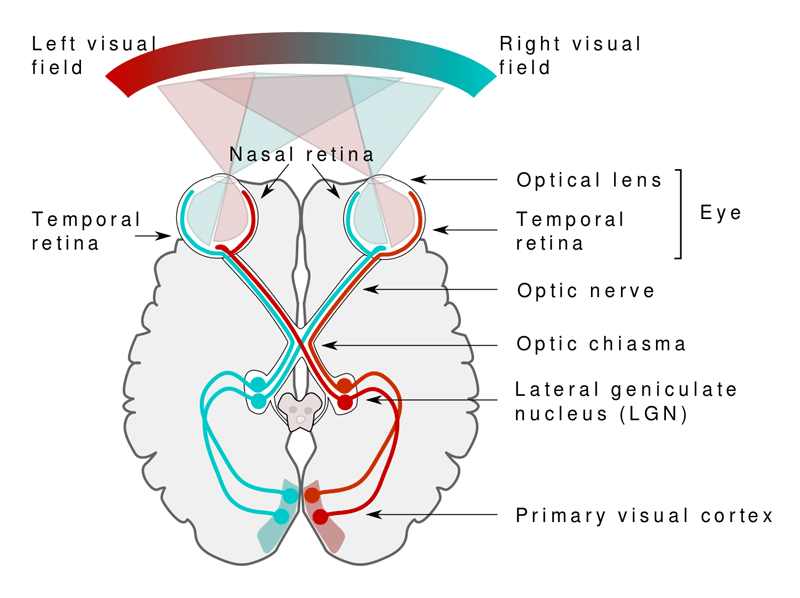
\includegraphics[height = 0.65 \textheight]{images/fig1.png}
        \caption{Program Timeline}
        \end{figure}
    \end{column}
    
    \begin{column}{0.4\textwidth}
    
    \begin{itemize}
      	\item<2-> sample: population \textbf<3->{\textcolor<3->{orange}{$<$450,000}}
      	\item<5-> selection by lottery
      	\item<6-> auditing process
      	\item<8-> audit report release
      \end{itemize}
    
    \only<3-4>{
    \begin{block}{\small \textbf{Important details}}
    \footnotesize
       \only<3-4>{\begin{itemize}
           \item<3-4> 92\% of all municipalities
           \item<3-4> 73\% of total population
           \item<4> excluding most state capitals/coastal cities
       \end{itemize}}
    \end{block}
    }
    
    \only<5>{
    \begin{block}{\small \textbf{Important details}}
    \footnotesize
       26 + 7$\times$50 + 5$\times$60 = 676 selections were made
       
       7 duplicated selections
       
       \textbf{669} municipalities were randomly selected 
    \end{block}
    }
    
    \only<6-7>{
    \begin{block}{\small \textbf{Important details}}
    \footnotesize
       \only<6-7>{\begin{itemize}
           \item<6-7> 10-15 auditors
           \item<6-7> 10 days of auditing
           \item<7> \textbf{validity}: hired competitively; well trained and paid; supervised
       \end{itemize}}
    \end{block}
    }
    
    \only<8-9>{
    \begin{block}{\small \textbf{Important details}}
    \footnotesize
       \only<8-9>{\begin{itemize}
           \item<8-9> reports: legislators/prosecutors
           \item<8-9> \textbf{summary}: \textbf<9>{\textcolor<9>{orange}{media}} and the Internet
           \item<9> {What form of media?} \textbf{\textcolor{orange}{radio}}
       \end{itemize}}
    \end{block}
    }
    
    \only<10-11>{\vspace{15pt}\textbf{\textcolor{orange}{Is the information really used by voters?}}}
    
    \only<11>{Yes, allegedly.}
    \end{column}
    \end{columns}
    \end{frame}
    
    \begin{frame}{\textit{Information:} The Measure of Corruption}
    
    \only<1-7>{
    \underline{What information is revealed on the audit reports}?
    \begin{itemize}
        \item<2-> \textbf{\textcolor{orange}{Quantitative:}} total amount of federal funds  transferred and the amount audited
        \item<3->\textbf{\textcolor{orange}{Qualitative:}} an itemized list describing each irregularity
    \end{itemize}}
    
    \begin{columns}[T]

    \begin{column}{0.3\textwidth}
        \uncover<4->{\begin{block}{\small \centering \textbf{Irregular procurement}}
        \uncover<5->{\footnotesize
        \begin{itemize}
            \item[-] no call for bids or minimum number of bids not attained
            \item[-] evidence of fraud
        \end{itemize}
        }
        \end{block}}
    \end{column}
    
    \begin{column}{0.3\textwidth}
        \uncover<4->{\begin{block}{\small \centering \textbf{Diversion of public funds}}
        \uncover<6->{\footnotesize
        \begin{itemize}
            \item[-] expenditure without proof
            \item[-] direct evidence of diversion
        \end{itemize}
        }
        \end{block}}
    \end{column}
    
    \begin{column}{0.3\textwidth}
        \uncover<4->{\begin{block}{\small \centering \textbf{Over-invoicing}}
        \uncover<7->{\footnotesize
        \begin{itemize}
            \item[-] purchase of public goods and services above the market price
        \end{itemize}
        }
        \end{block}}
    \end{column}
    
    \end{columns}
    
    \only<8->{
    \vspace{15pt}
    \underline{Construct a single measure}: the \textbf<9>{\textcolor<9>{orange}{total number of times}} each one of the three irregularities appears
    \begin{itemize}
        \small
        \item<10-> \textbf{\color{orange}Justification 1}: most common
        \item<11-> \textbf{\color{orange}Justification 2}: often complementary
        \item<12> {\footnotesize My interpretation: Layer 1 measure of corruption magnitude, could be more detailed, quantitatively}
    \end{itemize}
    }
        
    \end{frame}
    
    \begin{frame}{\textit{Political Consequence:} Municipal Election Results}
    \only<1->{
    \underline{Outcome: \textbf<2->{\textcolor<2->{orange}{Reelection results}}} 
    
    \begin{itemize}
        
        \item<3-> \textbf{\textcolor{orange}{Data source:}} Tribunal Superior Eleitoral (TSE)
        
        \item<3-> \textbf{\textcolor{orange}{Time frame:}} 2000 and 2004 voting results
        
        \item<3->
        \textbf{\textcolor{orange}{Voting information:}} Vote totals for each candidate by municipality
        
        \item<4-> \textbf{\textcolor{orange}{Sample selection:}} only first-term mayors eligible for reelection included
        
        \hspace*{\fill}\textbf<5->{(\textcolor<5->{orange}{373 municipalities}\only<5->{, 60\% of all mayors})}

    \end{itemize}}
        
    \end{frame}
    
    \begin{frame}{\textit{Covariates:} Candidate and Municipal Characteristics}
    \begin{itemize}
        \item<+-> Candidate characteristics from TSE
        \item<+-> Municipal characteristics from Brazilian Institute of Geography and Statistics (IBGE) 
        \begin{itemize}
            \item<+-> \textbf<6>{\textcolor<6>{orange}{2000}} population census: demographics
            \item<+-> \textbf<6>{\textcolor<6>{orange}{1999}} municipality survey: various controls
            \begin{itemize}
                \item public administration information: budgetary and planning procedures, public infrastructures, judiciary features, etc.
                \item measures of the \textbf<5->{\textcolor<5->{orange}{availability of media}}: the number of radio stations, daily newspapers, etc. 
            \end{itemize}
        \end{itemize}
        
    \end{itemize}
    
        
    \end{frame}
    
    %\section{Empirical Strategy}

 \frame{\sectionpage}

    \begin{frame}{Randomization Test}
        \only<1>{
            $$168\text{\ audited after election }v.s.\ 205\text{ audited before election}$$
        }

        \only<2>{
            $$\underbrace{168}_{\color{orange}C}\text{\ audited after election }v.s.\ \underbrace{205}_{\color{orange}T}\text{ audited before election}$$
        }
    \end{frame}
    
    \begin{frame}{Randomization Test: Political Characteristics}
        \only<1->{
            $$\underbrace{168}_{\color{orange}C}\text{\ audited after election }v.s.\ \underbrace{205}_{\color{orange}T}\text{ audited before election}$$
        }

        \uncover<1->{
        \begin{table}[h!]
            \footnotesize
            \begin{center}
              \label{tab:randomization1}
              \begin{tabular}{lcccc}
                
                & Control & Treatment & Difference & Std.Error \\
                \hline
                \textcolor<2>{orange}{Reelection rates: 2004 elections} & 0.413 & 0.395 & 0.018 & 0.045 \\
                \textcolor<3-4>{orange}{Reelection rates: 2000 elections \only<4>{(669 manicipalities)}} & 0.423 & 0.443 & -0.020 & 0.040 \\
                \textcolor<5>{orange}{2004 reelection rates, conditional on running} & 0.585 & 0.559 & 0.026 & 0.044 \\
                \textcolor<5>{orange}{Ran for reelection in 2004} & 0.707 & 0.707 & -0.001 & 0.060\\
                \textcolor<6>{orange}{Mayor's vote share in 2000} & 0.529 & 0.525 & 0.004 & 0.013
              \end{tabular}
            \end{center}
          \end{table}
        }
        
    \only<3-4>{
        No significant differences between C and T w.r.t. \textcolor<4>{orange}{\textit{natural}} reelection rates (among those eligible to re-run)
    }

    \only<4>{
        \footnotesize In 2000, every mayor was eligible to run for a second term, since only after 1997 it was allowed to run as an incumbent.
    }

    \only<5>{
        Balanced rate of re-running and incumbent advantage
    }

    \only<6>{
        Initial popularity of reelection seeking mayors is balanced too
    }

    \end{frame}

    \begin{frame}{Randomization Test: Mayor and Municipal Characteristics}
        \only<1->{
            $$\underbrace{168}_{\color{orange}C}\text{\ audited after election }v.s.\ \underbrace{205}_{\color{orange}T}\text{ audited before election}$$
        }

        \uncover<1->{
        \begin{table}[h!]
            \footnotesize
            \begin{center}
              \label{tab:randomization2}
              \begin{tabular}{lcccc}
                
                & Control & Treatment & Difference & Std.Error \\
                \hline
                \multicolumn{5}{l}{\textit{Panel A: Mayor characteristics}}\\
                Member of PMDB & 0.254 & 0.172 & \textcolor<2>{orange}{0.082} & \textcolor<2>{orange}{0.047} \\
                &\\
                \multicolumn{5}{l}{\textit{Panel B: Municipal characteristics}}\\
                Number of newspapers & 3.58 & 2.21 & \textcolor<2>{orange}{1.37} & \textcolor<2>{orange}{0.79} \\
                Share of HHs that own a radio & 0.423 & 0.443 & -0.020 & 0.040 \\
                \textcolor<3>{orange}{Municipalities with a radio station} & 0.585 & 0.559 & 0.026 & 0.044 \\
                \textcolor<3>{orange}{Number of radio stations (condtional on having one)} & 0.707 & 0.707 & -0.001 & 0.060
              \end{tabular}
            \end{center}
          \end{table}
        }

        \only<3>{
        Radio presence is well-balanced.
        }

    \end{frame}

    \begin{frame}{Randomization Test: Constructed Corruption Measure}
        \only<1->{
            $$\underbrace{168}_{\color{orange}C}\text{\ audited after election }v.s.\ \underbrace{205}_{\color{orange}T}\text{ audited before election}$$
        }

        \uncover<1->{
        \begin{table}[h!]
            \footnotesize
            \begin{center}
              \label{tab:randomization3}
              \begin{tabular}{lcccc}
                
                & Control & Treatment & Difference & Std.Error \\
                \hline
                Number of corrupt violations & 1.952 & 1.584 & 0.369 & 0.357 \\
                Total resources audited (R\$) &  5,770,189 & 5,270,001 & 500,188 & 1,361,431
              \end{tabular}
            \end{center}
          \end{table}
        }

        \only<2>{
        The constructed measure is balanced, so is the \textit{intensity} of auditing.
        }

    \end{frame}
    
    
    \begin{frame}{Randomization Test: Constructed Corruption Measure}
        \begin{figure}\label{fig2}
            \centering
            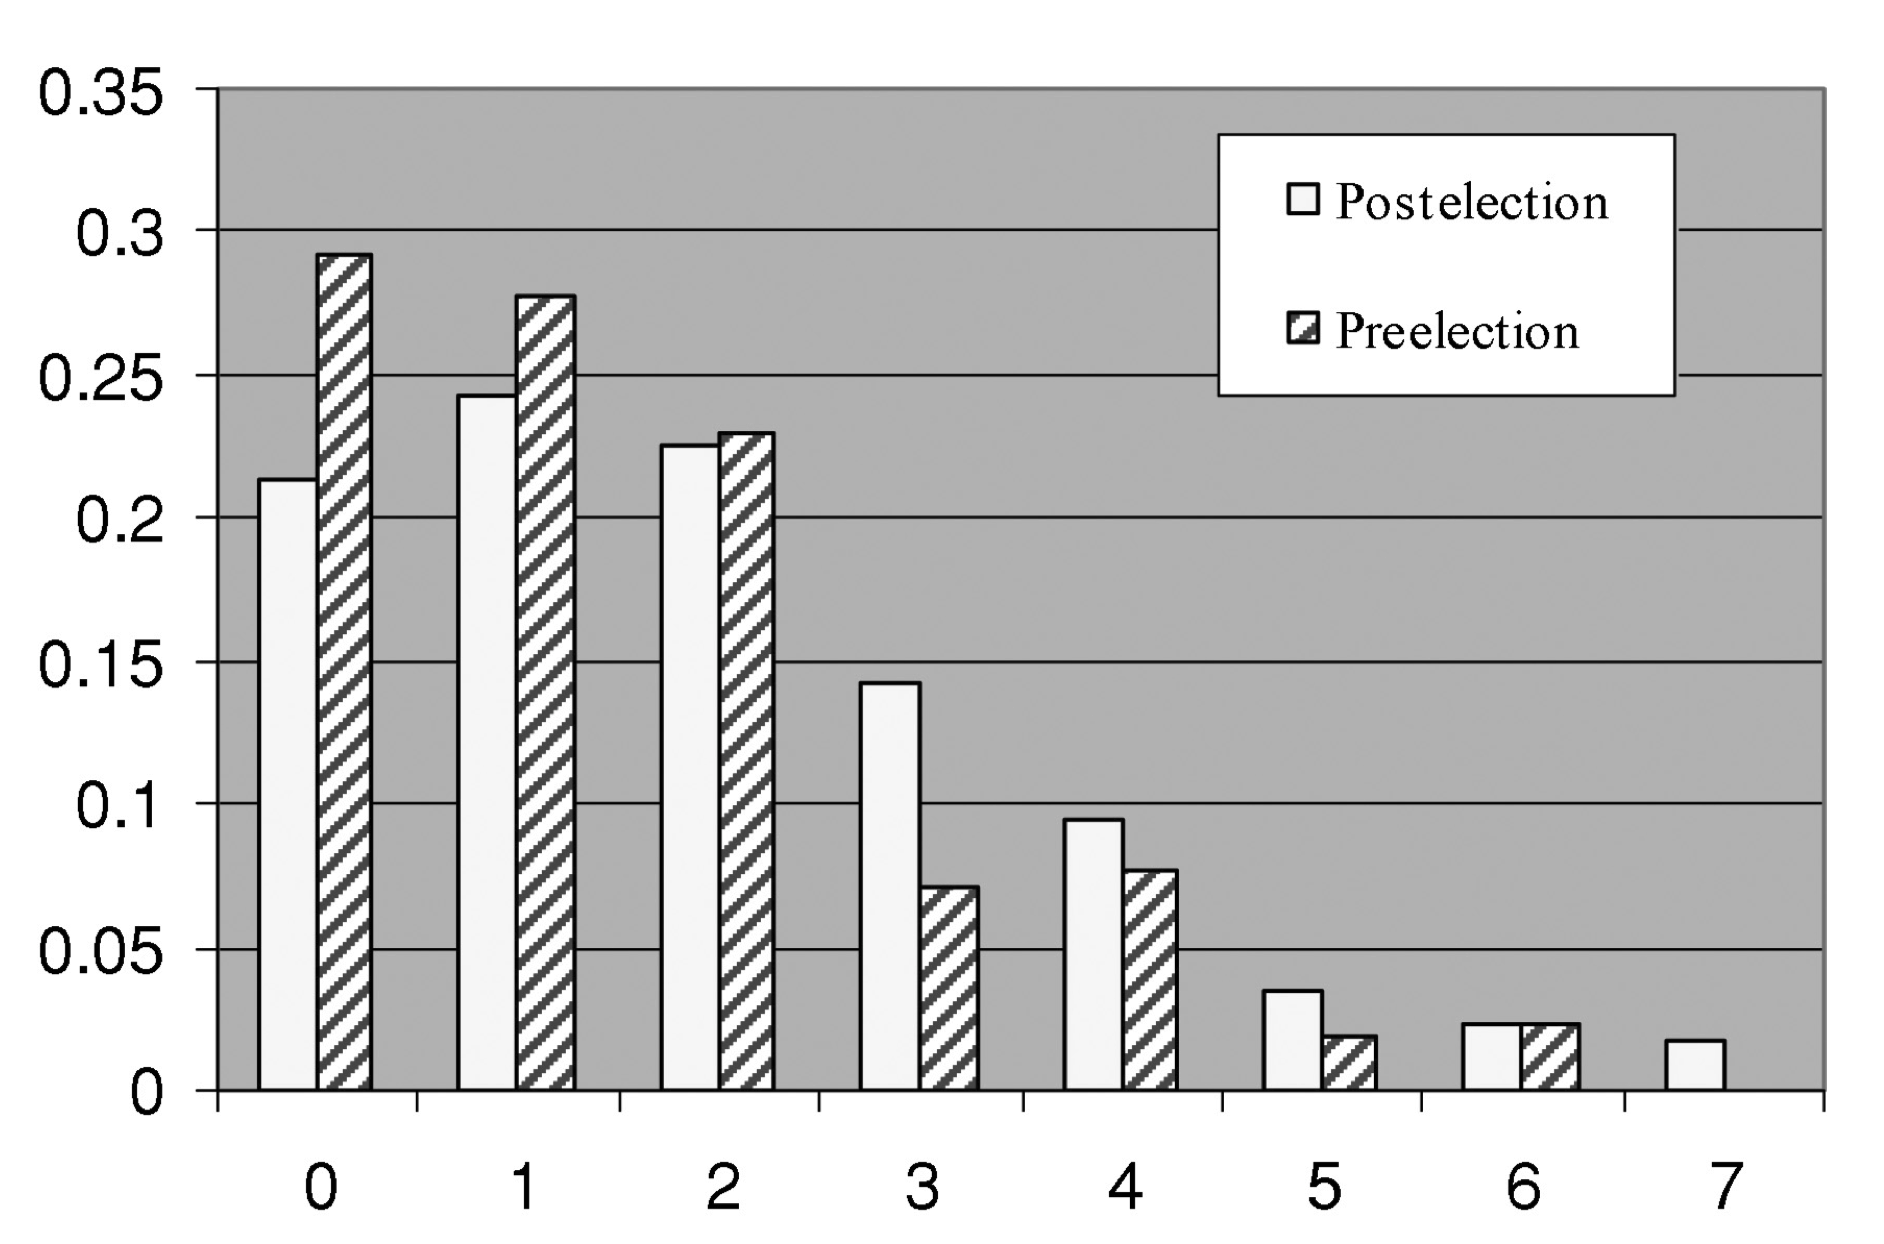
\includegraphics[height = 0.65 \textheight]{images/fig2.png}
            \caption{Distribution of Corrupt Violations}
            \end{figure}
    \end{frame}

\begin{frame}{Estimation I: Exogenous Treatment}
\only<1->{
    \begin{equation*}
        \textcolor<2-3>{orange}{E_{ms}} = \alpha + \textcolor<7>{orange}{\beta} \textcolor<4>{orange}{A_{ms}} + \textcolor<5>{orange}{X_{ms}}\gamma + \textcolor<6>{orange}{\nu_s}+ \epsilon_{ms}
    \end{equation*}
}

\only<2->{
    where:
    \begin{itemize}
        \small
        \item<2-> {\color{orange} $E_{ms}$}: reelection performance of an eligible incumbent mayor in {\color{orange}\textbf{municipality} $m$}, {\color{orange}\textbf{state} $s$}
        \only<3>{
            \begin{itemize}
                \footnotesize
                \item[-] Discrete: whether winning the reelection or not
                \item[-] Continuous: vote share; win margin
                \item[-] Changes from 2000 results: $\Delta E_{ms}=E_{ms,2004}-E_{ms,2000}$
            \end{itemize}
        }
        \item<4-> {\color{orange} $A_{ms}$}: $=1$ if audited prior to the 2004 elections
        \item<5-> {\color{orange} $X_{ms}$}: municipality and mayor controls
        \item<6-> {\color{orange} $\nu_s$}: state fixed effect 
    \end{itemize}
}

\only<7>{
    {\color{orange} $\beta$}: the treatment effect of \underline{being audited and the public release of auditing results}
}
    
\end{frame}

\begin{frame}{Estimation II: Adding Voters' Prior Beliefs}
    \only<1->{
    \begin{equation*}
        E_{ms} = \alpha + \only<2->{ \beta_0 \textcolor<3>{orange}{C_{ms}} +} \beta_1 A_{ms} \only<2->{+ \textcolor<4->{orange}{\beta_2} \textcolor<3>{orange}{\left(A_{ms}\times C_{ms}\right)} } + X_{ms}\gamma + \nu_s + \epsilon_{ms}
    \end{equation*}
    }
    
    \only<3->{
    where:
    \begin{itemize}
        \small
        \item<3-> {\color{orange} $C_{ms}$}: {\color{orange}\textbf{number of}} corrupt irregularities in the municipality
        \item<3-> {\color{orange} $A_{ms}\times C_{ms}$}: interaction term 
    \end{itemize}

}

\only<4->{
    {\color{orange} $\beta_2$}: the treatment effect conditional on corruption levels
    \only<5->{
        \begin{itemize}
            \small
            \item<5-> \textbf{\color{orange}Prediction}: Negative treatment effect at higher levels of reported corruption, presumably positive at lower levels.
            \item<6> \textbf{\color{orange}Underlying assumption}: Voters do \textbf{\color{orange}not} systematically over- or underestimate the incumbent's corruption level.
        \end{itemize}
    }
}

\end{frame}

\begin{frame}{Estimation III: Adding the Presence of Local Media}
    \only<1>{
        \begin{equation*}
            E_{ms} = \alpha + \beta_0 C_{ms} + \beta_1 A_{ms} + \beta_2 \left(A_{ms}\times C_{ms}\right) + X_{ms}\gamma + \nu_s + \epsilon_{ms}
        \end{equation*}
    }
    \only<2->{
        \begin{align*}
            E_{ms} =& \alpha + \beta_0C_{ms} + \beta_1 A_{ms} + \beta_2\textcolor<3>{orange}{ M_{ms}} + \beta_3\textcolor<5>{orange}{ \left(A_{ms}\times M_{ms}\right)} + \beta_4\left(A_{ms}\times C_{ms}\right)\\
            & + \beta_5\textcolor<5>{orange}{\left(M_{ms}\times C_{ms}\right)} + \textcolor<7>{orange}{\beta_6}\textcolor<6>{orange}{\left( A_{ms}\times C_{ms}\times M_{ms} \right)} + X_{ms}\gamma+\nu_s +\epsilon_{ms}
        \end{align*}
    }
        
        \only<3->{
        where:
        \begin{itemize}
            \small
            \item<3-> {\color{orange} $M_{ms}$}: measure of media presence
            \only<4>{
                \begin{itemize}
                    \item[-] main specification: the number of local \textbf{\color{orange}AM radio stations}
                    \item[-] robustness check: share of HHs with radios, number of newspapers, share of HHs with a TV
                \end{itemize}
            }
            \item<5-> {\color{orange} $A_{ms}\times M_{ms},M_{ms}\times C_{ms}$}: double interaction terms 
            \item<6-> {\color{orange} $A_{ms}\times C_{ms}\times M_{ms}$}: triple interaction terms 
        \end{itemize}
    
    }
    
    \only<7>{
        {\color{orange} $\beta_6$}: the treatment effect conditional on corruption levels and local media presence
    }
    
\end{frame}

\begin{frame}{Estimations: Summary}
    \begin{align*}
        E_{ms} =& \alpha + \textcolor<2->{orange}{\beta}A_{ms} + \textcolor<5>{orange}{X_{ms}}\gamma + \nu_s+ \epsilon_{ms} &(1)\\
        E_{ms} =& \alpha + \beta_0 C_{ms} + \beta_1 A_{ms} + \textcolor<3->{orange}{\beta_2} \left(A_{ms}\times C_{ms}\right) + \textcolor<5>{orange}{X_{ms}}\gamma + \nu_s + \epsilon_{ms} & (2)\\
        E_{ms} =& \alpha + \beta_0C_{ms} + \beta_1 A_{ms} + \beta_2 M_{ms} + \beta_3 \left(A_{ms}\times M_{ms}\right) + \beta_4\left(A_{ms}\times C_{ms}\right)\\
        & + \beta_5 \left(M_{ms}\times C_{ms}\right) + \textcolor<4->{orange}{\beta_6} \left( A_{ms}\times C_{ms}\times M_{ms} \right) + \textcolor<5>{orange}{X_{ms}}\gamma+\nu_s +\epsilon_{ms} & (3)
    \end{align*}

    \begin{itemize}
        \small
        \item<2-> $\beta$: Average treatment effect of pre-election auditing
        \item<3-> $\beta_2$: Treatment effect, conditional on \textcolor<3->{orange}{corruption level}
        \item<4-> $\beta_6$: Treatment effect, conditional on \textcolor<4->{orange}{corruption level and media presence}
        \item<5-> $X_{ms}$: Controls should \textbf{\color{orange}not} have an effect
    \end{itemize}
    
\end{frame}

    %\section{Results}

 \frame{\sectionpage}

\begin{frame}{Estimation I: Exogenous Treatment}
\only<1->{
    \small
    \begin{equation*}
        E_{ms} = \alpha + \textcolor{orange}{\beta}A_{ms} + X_{ms}\gamma + \nu_s+ \epsilon_{ms}
    \end{equation*}
}

\uncover<1->{
    \begin{table}[h!]
        \footnotesize
        \begin{center}
            \label{tab:result1}
            \begin{tabular}{lcccc}
            
            & \multicolumn{2}{c}{All incumbent mayors} & & Those ran \\
            & (1) & (2) & & (3) \\
            \hline
            Preelection audit (1/0) & \textcolor<2-3>{orange}{-0.036} & \textcolor<2-4>{orange}{0.036} & & \textcolor<2,4>{orange}{-0.059} \\
             & \textcolor<2-3>{orange}{(0.053)} & \textcolor<2-4>{orange}{(0.052)} & & \textcolor<2,4>{orange}{(0.065)}\\
             Observations & 373 & 373 &  & 263\\
             $R^2$ & 0.05 & 0.17 & & 0.22\\
             State FEs & Yes & Yes & & Yes\\
             Municipal controls & \textcolor<3>{orange}{No} & \textcolor<3>{orange}{Yes} & & Yes \\
             Mayoral controls & \textcolor<3>{orange}{No} & \textcolor<3>{orange}{Yes} & & Yes
            \end{tabular}
        \end{center}
        \end{table}

    {\footnotesize \textbf{\color{orange} Note:} Hereafter, robust standard errors are displayed in parenthesis, significant levels: 99\%(**), 95\%(*), 90\%(+).}
    }
    
\end{frame}

\begin{frame}{Estimation I: Exogenous Treatment}
    \only<1->{
    \small
    \begin{equation*}
        E_{ms} = \alpha + \textcolor{orange}{\beta}A_{ms} + X_{ms}\gamma + \nu_s+ \epsilon_{ms}
    \end{equation*}
}

\uncover<1->{
    \begin{table}[h!]
        \footnotesize
        \begin{center}
            \label{tab:result2}
            \begin{tabular}{lccccc}
            
            \multicolumn{6}{c}{Only mayors ran for reelection}\\
            \hline
            & Pr(reelection) & Vote share & Win margin & $\Delta$vote share & $\Delta$win margin \\
            & (3) & (4) & (5) & (6) & (7) \\
            \hline
            Preelection audit (1/0) & -0.059 & -0.055 & -0.020 & -0.032$^{+}$ & -0.028 \\
             & (0.065) & (0.072) & (0.027) & (0.018) & (0.027)\\
             Observations & 263 & 263 & 263 & 263 & 263\\
             $R^2$ & 0.22 & 0.16 & 0.22 & 0.39 & 0.31 \\
             State FEs & \multicolumn{5}{c}{Yes}\\
             Municipal controls  & \multicolumn{5}{c}{Yes} \\
             Mayoral controls  & \multicolumn{5}{c}{Yes}
            \end{tabular}
        \end{center}
        \end{table}

    }
\end{frame}

\begin{frame}{Estimation I: Exogenous Treatment}
    \only<1->{
    \small
    \begin{equation*}
        E_{ms} = \alpha + \textcolor{orange}{\beta}A_{ms} + X_{ms}\gamma + \nu_s+ \epsilon_{ms}
    \end{equation*}
}

Results: $\beta=0$

\vspace*{20pt}

\begin{enumerate}
    \small
    \item<2-> \textbf{\color{orange}Beliefs} matter: The effects of surprisingly low and high levels of corruption cancel each other out.
    \item<3-> \textbf{\color{orange}Media presence} matters: Information might not be so effectively disseminated.
\end{enumerate}
    
\end{frame}

\begin{frame}{Estimation II: Adding Voters' Prior Beliefs}
    \begin{figure}\label{fig3}
        \centering
        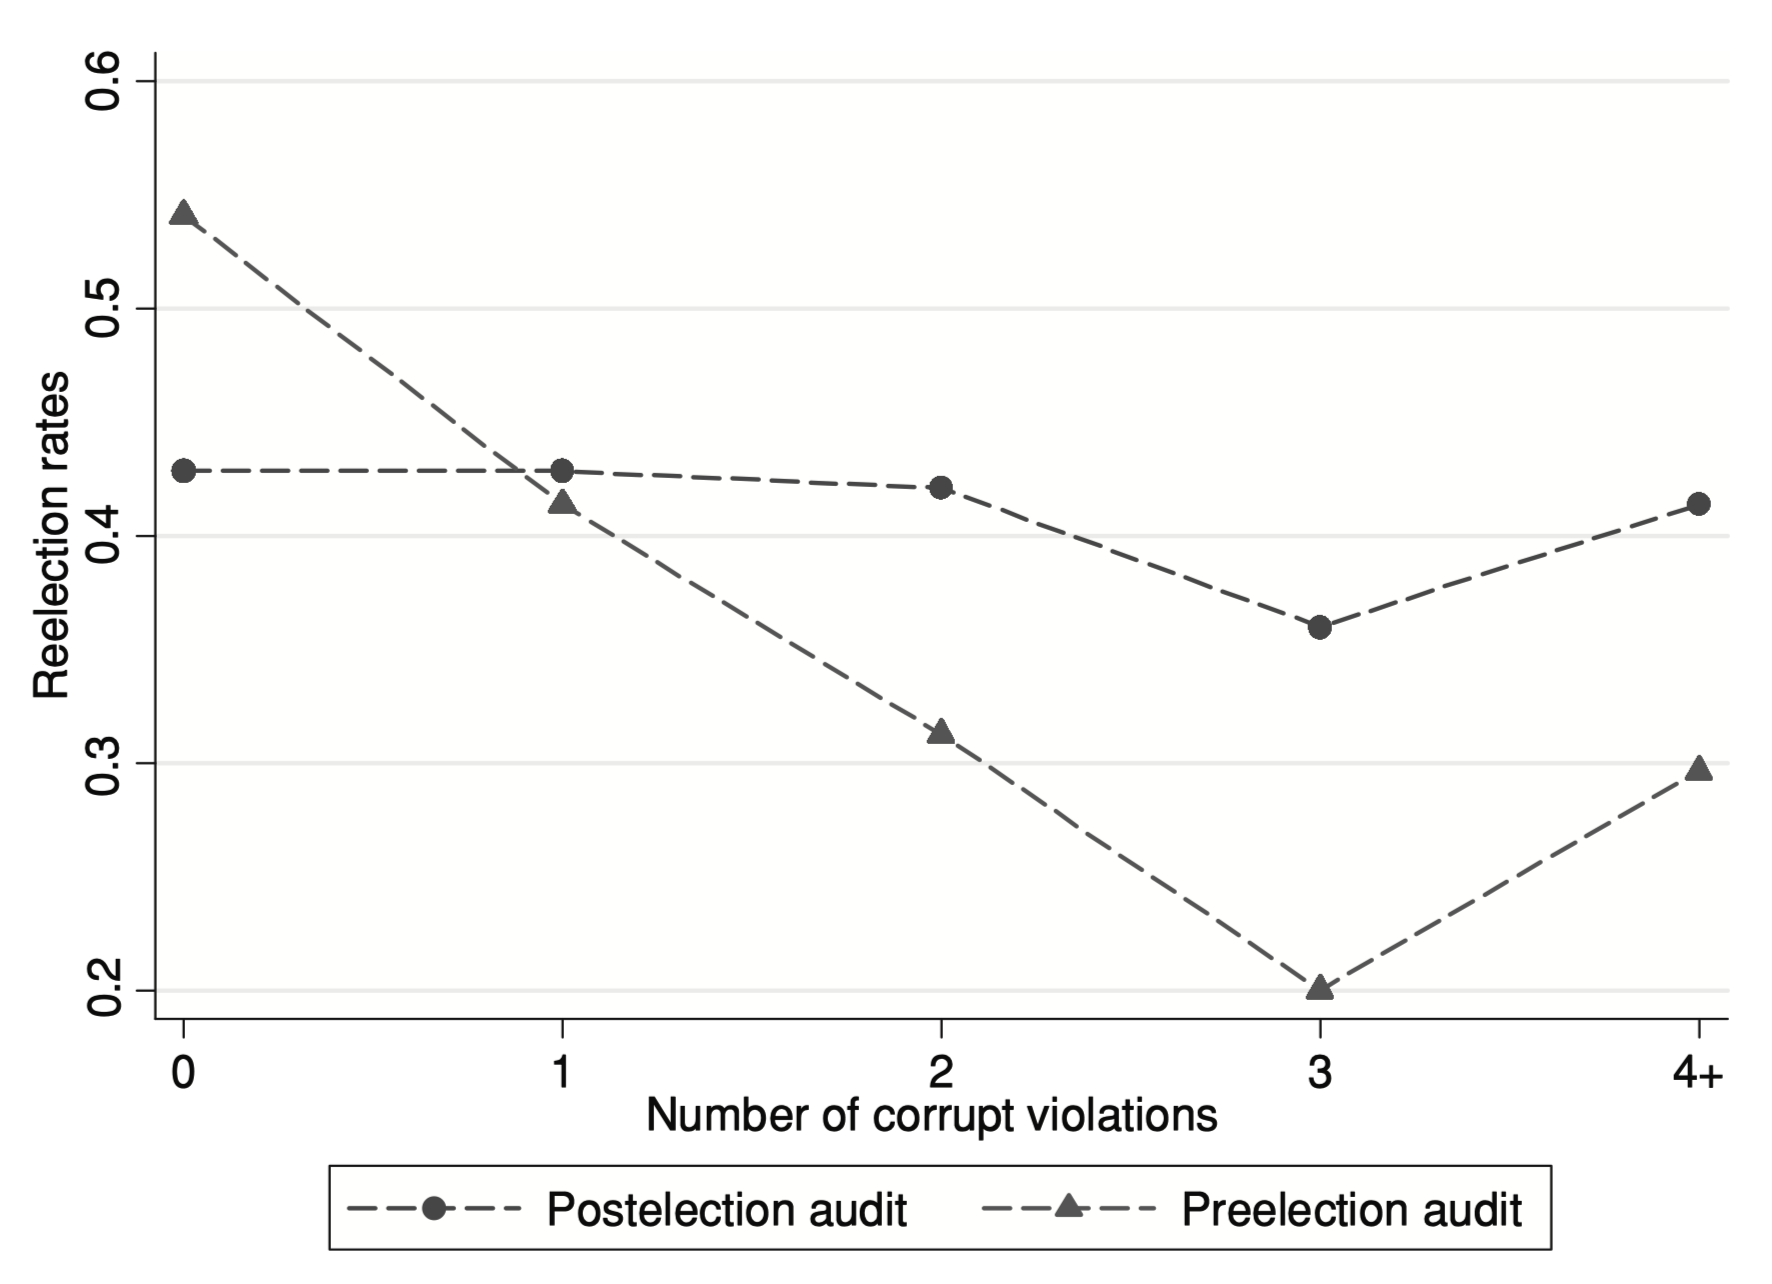
\includegraphics[height = 0.65 \textheight]{images/fig3.png}
        \caption{Descriptive evidence: Reelection Rates and Corruption Levels}
        \end{figure}
\end{frame}

\begin{frame}{Estimation II: Adding Voters' Prior Beliefs}

    \only<1>{
            \footnotesize
            \begin{align*}
                E_{ms} =& \alpha + \beta_0 C_{ms} + \beta_1 A_{ms} + \textcolor{orange}{\beta_2} \left(A_{ms}\times C_{ms}\right) + X_{ms}\gamma + \nu_s + \epsilon_{ms}
            \end{align*}
            }

    \begin{columns}

        \begin{column}{0.4\textwidth}
            \begin{figure}
            \centering
            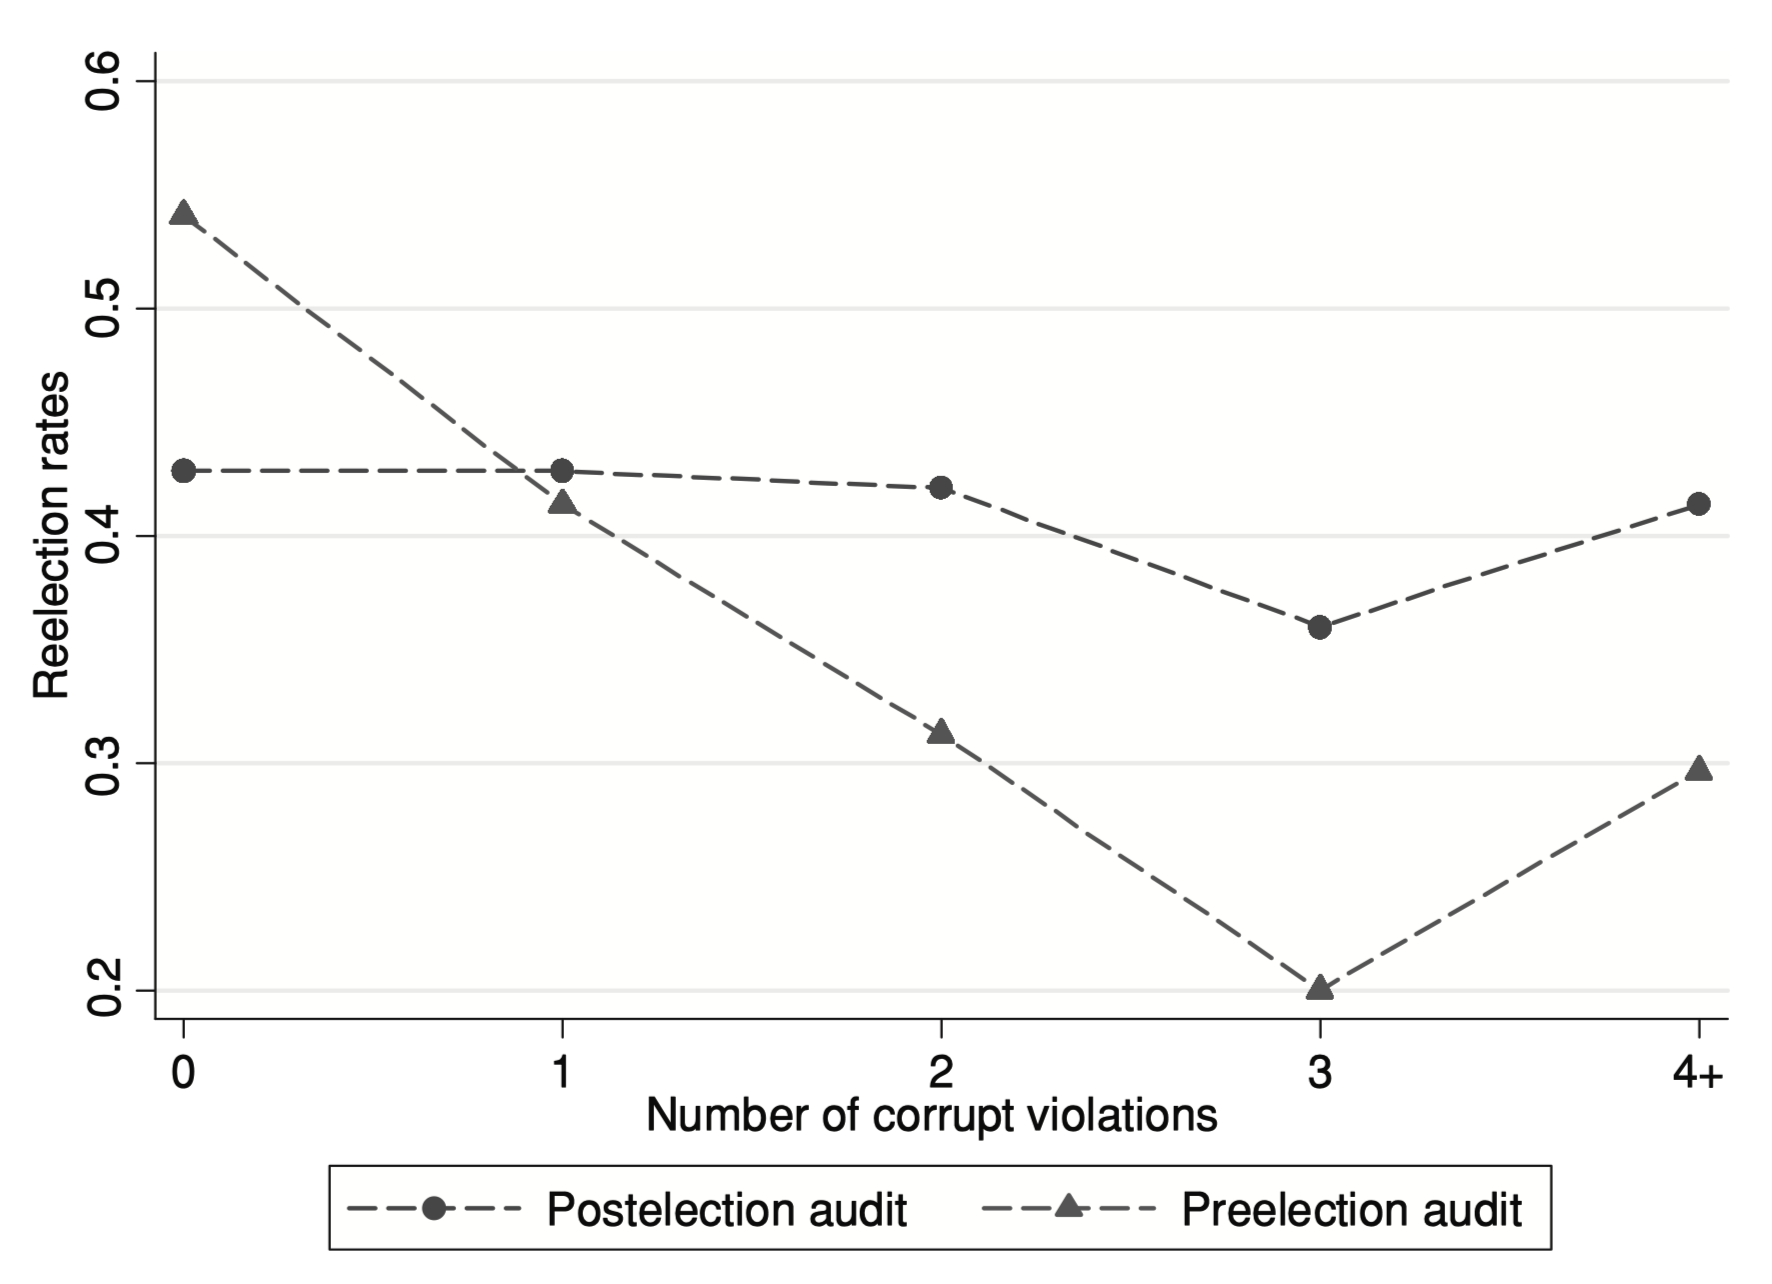
\includegraphics[height = 0.55 \textheight]{images/fig3.png}
            \end{figure}
        \end{column}

        \begin{column}{0.55\textwidth}

            \only<2->{
                \begin{table}[h!]
                    \footnotesize
                    \begin{center}
                        \label{tab:result2-1}
                        \begin{tabular}{lcc}
                        
                        \multicolumn{3}{c}{\color{orange}Linear}\\
                        & (1) & (2) \\
                        \hline
                        Preelection audit $\times$ & -0.038 & -0.038 \\
                         No. corruption violations & (0.035) & (0.035) \\
                         & \\
                         Observations & 373 & 373 \\
                         $R^2$ & 0.05 & 0.18\\
                         State FEs & Yes & Yes\\
                         Municipal controls & \textcolor{orange}{No} & \textcolor{orange}{Yes} \\
                         Mayoral controls & \textcolor{orange}{No} & \textcolor{orange}{Yes} 
                        \end{tabular}
                    \end{center}
                    \end{table}
            }
        
        \end{column}

    \end{columns}

\end{frame}

\begin{frame}{Estimation II: Adding Voters' Prior Beliefs}

    \begin{columns}

        \begin{column}{0.4\textwidth}
            \begin{figure}
            \centering
            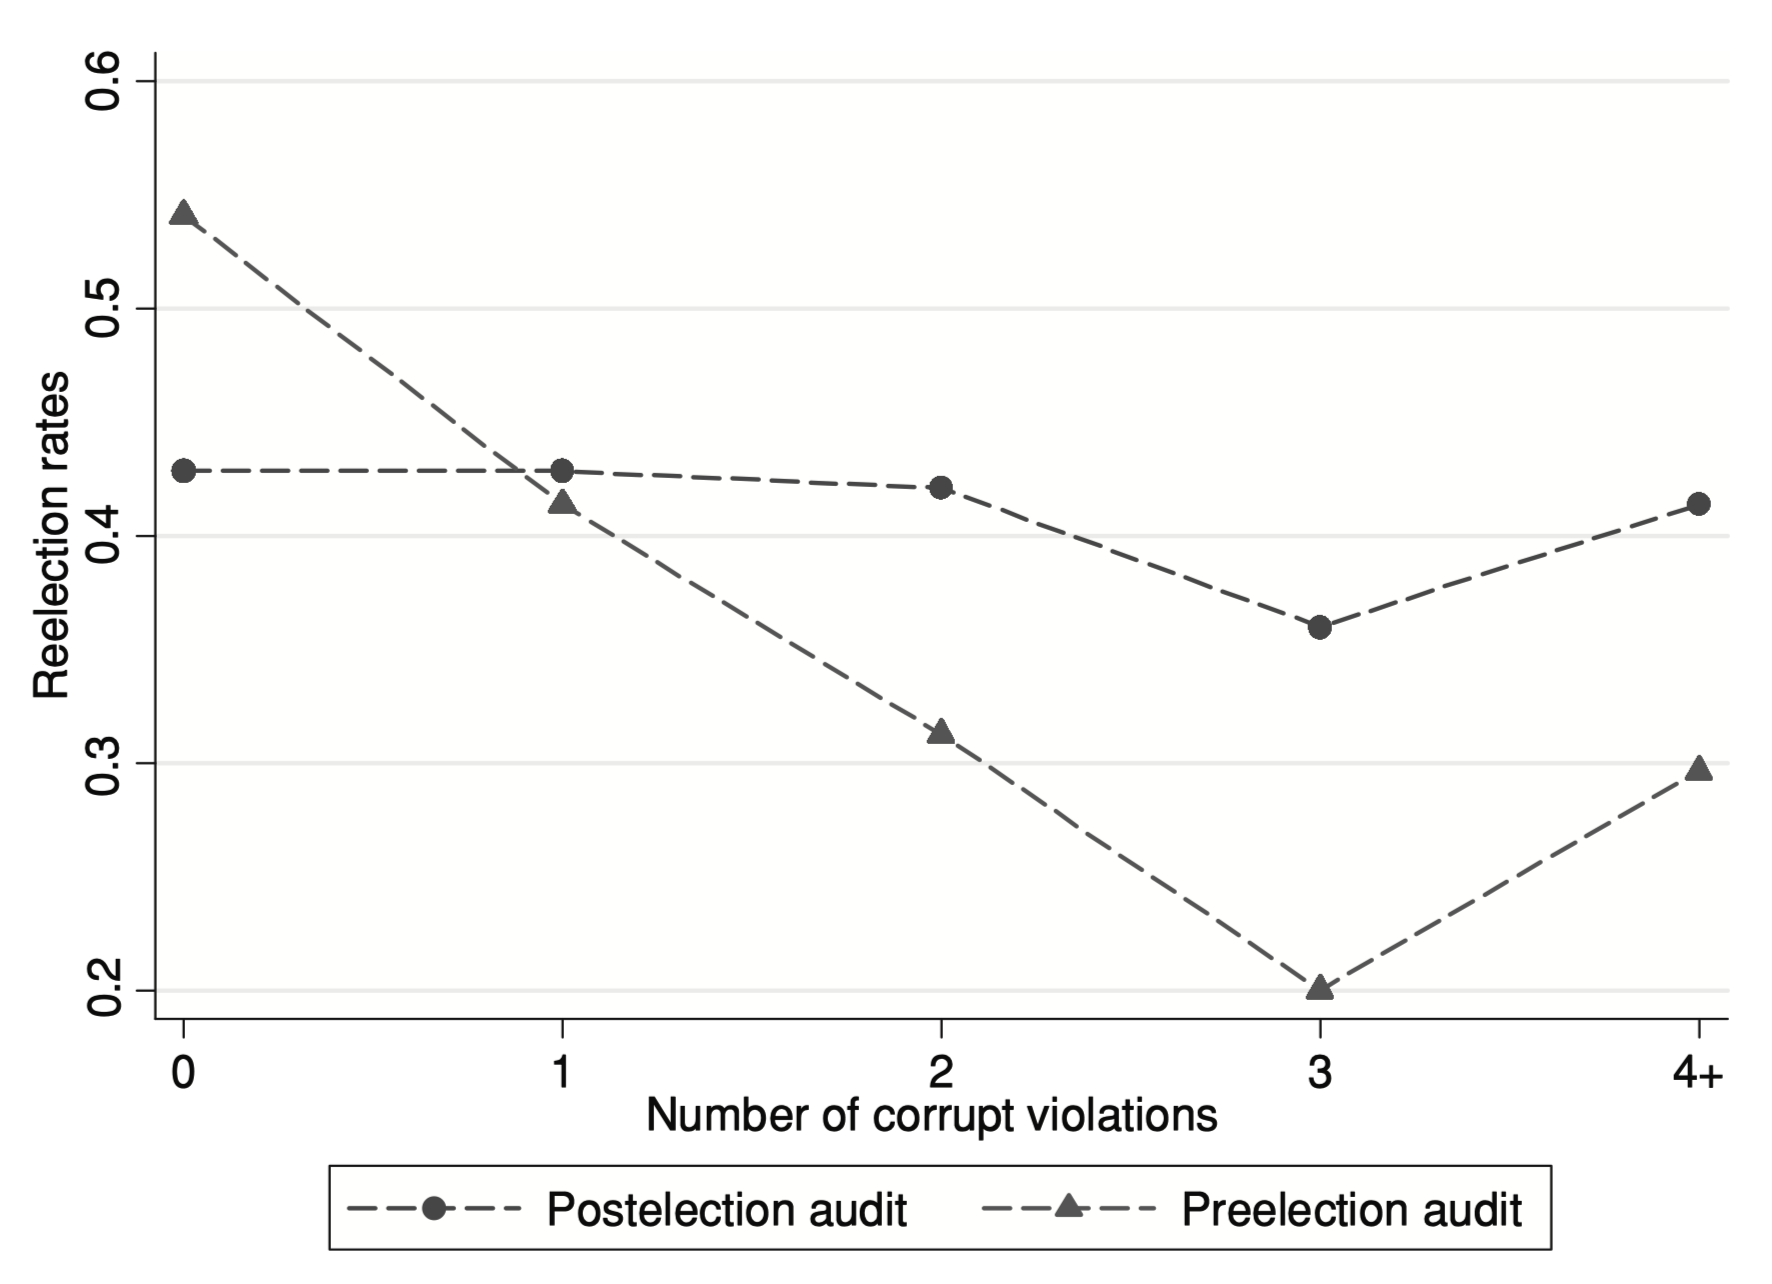
\includegraphics[height = 0.55 \textheight]{images/fig3.png}
            \end{figure}
        \end{column}

        \begin{column}{0.55\textwidth}

            \only<1->{
                \begin{table}[h!]
                    \tiny
                    \begin{center}
                        \label{tab:result2-2}
                        \begin{tabular}{lccc}
                        
                        \multicolumn{4}{c}{Different models}\\
                        \hline
                        & Linear & \textcolor<2>{orange}{Quadratic} & \textcolor<3>{orange}{Semiparametric} \\
                        & (2) & (3) & (4)\\
                        \hline
                        Preelection audit $\times$ & -0.038 & \textcolor<2>{orange}{-0.200$^*$} & \\
                         No. corruption violations & (0.035) & (0.090) & \\
                         Preelection audit $\times$ &  & \textcolor<2>{orange}{0.034$^*$} &\\
                         No. corruption violations$^2$ & & (0.017) &\\
                         
                         Preelection audit $\times$ &  & & 0.010\\
                         corruption = 0 & & & (0.156)\\
                         Preelection audit $\times$ &  & &  \textcolor<3>{orange}{-0.253$^+$}\\
                         corruption = 2 & & & (0.148)\\
                         Preelection audit $\times$ &  &  & \textcolor<3>{orange}{-0.321$^+$}\\
                         corruption = 3 & & & (0.192)\\
                         Preelection audit $\times$ &  &  & -0.159\\
                         corruption = 4 & & & (0.168)\\
                         & \\
                         $R^2$ & 0.18 & \textcolor<2>{orange}{0.19} & \textcolor<3>{orange}{0.22} \\
                         $F-$test ($p$-value) & & \textcolor<2>{orange}{0.089} & \textcolor<3>{orange}{0.192}
                        \end{tabular}
                    \end{center}
                    \end{table}
            
            }
        
        \end{column}

    \end{columns}

\end{frame}

\begin{frame}{Estimation II: Adding Voters' Prior Beliefs}

    \begin{columns}

        \begin{column}{0.4\textwidth}
            \begin{figure}
            \centering
            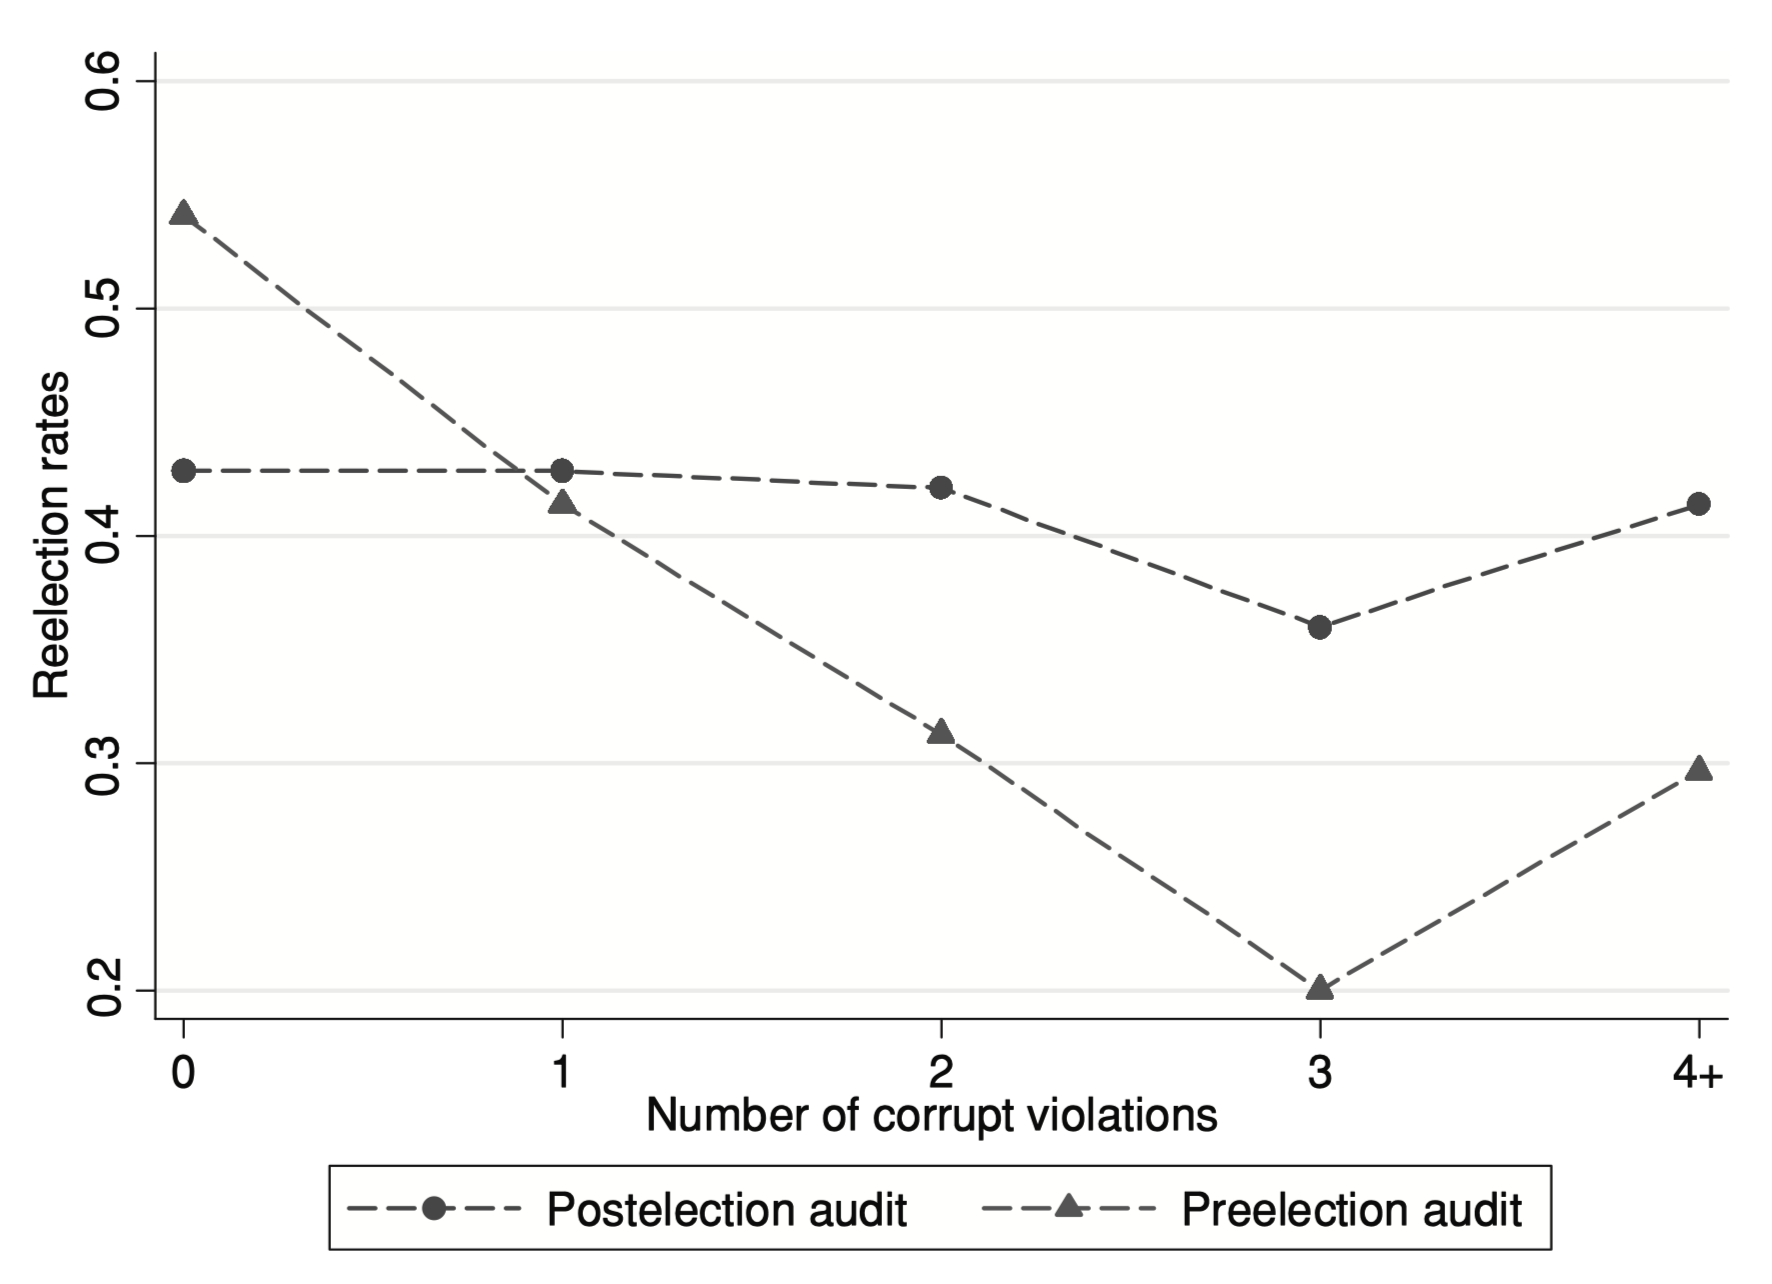
\includegraphics[height = 0.55 \textheight]{images/fig3.png}
            \end{figure}
        \end{column}

        \begin{column}{0.55\textwidth}

            \only<1->{
                \begin{table}[h!]
                    \tiny
                    \begin{center}
                        \label{tab:result2-3}
                        \begin{tabular}{lccc}
                        
                        \multicolumn{4}{c}{Different samples}\\
                        \hline
                        & Full & \textcolor<2>{orange}{Corruption$\leq$5} & \textcolor<3>{orange}{Corruption$\leq$4} \\
                        & (2) & (5) & (6)\\
                        \hline
                        Preelection audit $\times$ & -0.038 & \textcolor<2>{orange}{-0.070$^+$} & \textcolor<3>{orange}{-0.088$^*$} \\
                         No. corruption violations & (0.035) & (0.041) & (0.043)\\
                         & \\
                         Observations & 373 & \textcolor<2>{orange}{362} & \textcolor<3>{orange}{351} \\
                         $R^2$ & 0.18 & 0.19 & 0.20
                        \end{tabular}
                    \end{center}
                    \end{table} 
            
            }
        
        \end{column}

    \end{columns}

\end{frame}

\begin{frame}{Estimation II: Adding Voters' Prior Beliefs}

    \begin{columns}

        \begin{column}{0.4\textwidth}
            \begin{figure}
            \centering
            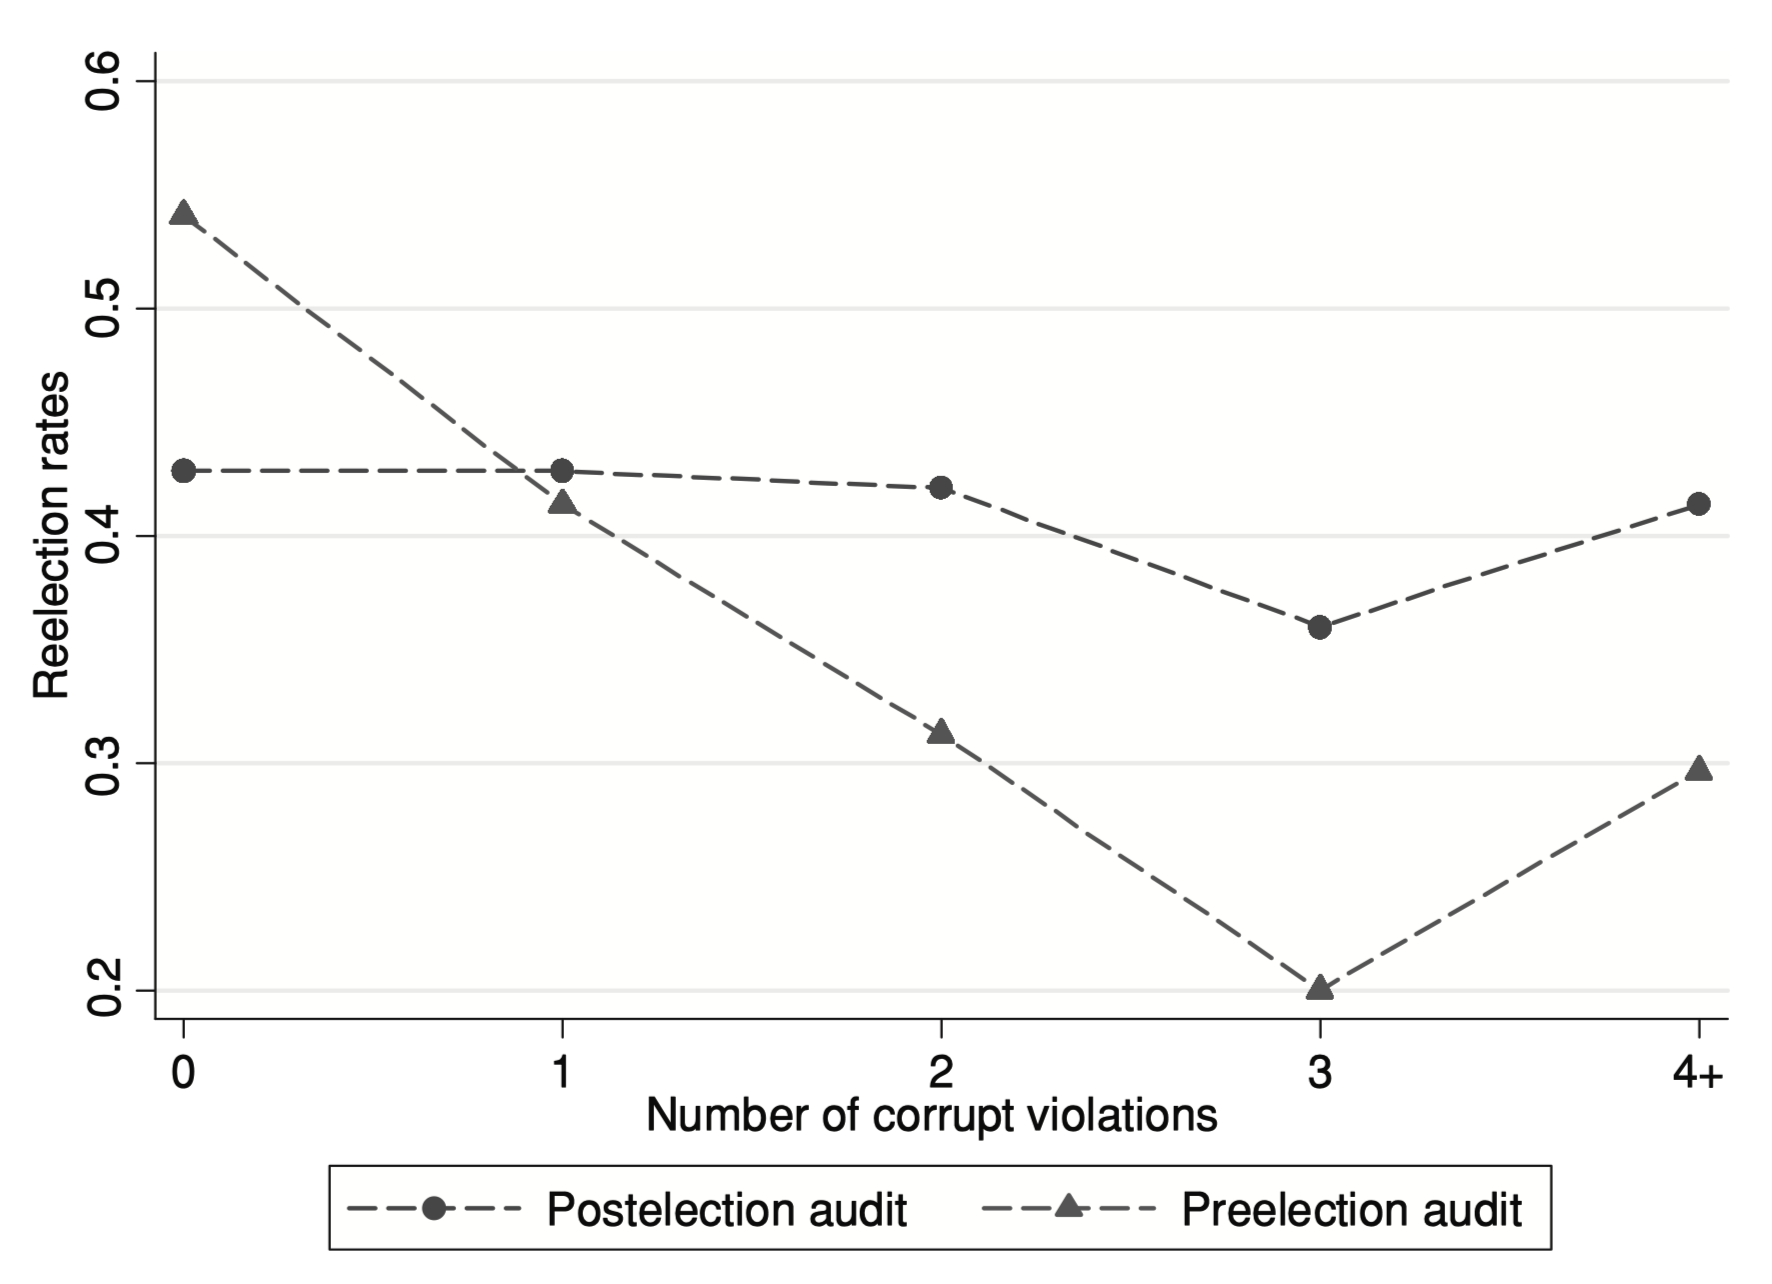
\includegraphics[height = 0.55 \textheight]{images/fig3.png}
            \end{figure}
        \end{column}

        \begin{column}{0.5\textwidth}

        \only<1->{
        \begin{block}{\small \textbf{Summary}}
        \footnotesize

            \only<1->{
                \begin{enumerate}
                    \item<2-> Model selection: The U-shape relationship is more likely driven by \textbf{\color{orange}noise}
                    \item<3-> Preferred specification: \textbf{\color{orange} Linear}, with the sub-sample of \textbf{\color{orange}Corruption$\leq$5} 
                    \item<4-> Estimation results: Marginal treatment effect per corruption violation is \textbf{\color{orange}-7\%} {\scriptsize (or \textbf{\color{orange}-16\%} of the 43\% control-group reelection rate)}.
                    \item<5-> Prior belief: Incumbents on average commit \textbf{\color{orange}1} corrupt violation 
                \end{enumerate}
            }
        \end{block}
        }

        \only<6>{\scriptsize
            \textbf{\color{orange}Question}: what about those extremely corrupted mayors?
        }
        
        \end{column}

    \end{columns}

\end{frame}


\begin{frame}{Estimation III: Adding the Presence of Local Media}
    \only<1->{
        \tiny
        \begin{align*}
        E_{ms} =& \alpha + \beta_0C_{ms} + \beta_1 A_{ms} + \textcolor<5>{orange}{\beta_2} M_{ms} + \textcolor<3>{orange}{\beta_3} \left(A_{ms}\times M_{ms}\right) + \beta_4\left(A_{ms}\times C_{ms}\right)\\
        & + \textcolor<4>{orange}{\beta_5} \left(M_{ms}\times C_{ms}\right) + \textcolor<2>{orange}{\beta_6} \left( A_{ms}\times C_{ms}\times M_{ms} \right) + X_{ms}\gamma+\nu_s +\epsilon_{ms}
        \end{align*}
    }

    \only<1->{
        \begin{table}[h!]
            \scriptsize
            \begin{center}
                \label{tab:result3-1}
                \begin{tabular}{lcccc}
                
                %\multicolumn{5}{c}{Dependent variable: Pr(reelection)}\\
                %\hline
                & & & & Demographics\\
                & Full & Corruption$\leq$5 & Demographics &  \& institutional  \\
                & (1) & (2) & (3) & (4) \\
                \hline
                 Preelection audit & -0.059 & -0.033 & 0.296 & 0.208 \\
                 No. corrupt violations & -0.034 & -0.013 & -0.13 & -0.069\\
                 No. radio stations & \textcolor<5>{orange}{-0.131$^*$} & \textcolor<5>{orange}{-0.150$^*$} & \textcolor<5>{orange}{-0.216$^{**}$} & \textcolor<5>{orange}{-0.253$^{**}$}\\
                 &\\
                 Preelection audit $\times$ No. radio stations & \textcolor<3>{orange}{0.229$^*$} & \textcolor<3>{orange}{0.271$^{**}$} & \textcolor<3>{orange}{0.356$^{**}$} & \textcolor<3>{orange}{0.449$^{**}$} \\
                 Preelection audit $\times$ No. corrupt violations & 0.007 & -0.018 & -0.236 & -0.412 \\
                 No. radio stations $\times$ No. corrupt violations & \textcolor<4>{orange}{0.050$^{+}$} & \textcolor<4>{orange}{0.058$^*$} & \textcolor<4>{orange}{0.082$^{**}$} &\textcolor<4>{orange}{0.09$^{**}$}\\
                 &\\
                 Triple interaction & \textcolor<2>{orange}{-0.118$^{**}$} & \textcolor<2>{orange}{-0.157$^*$} & \textcolor<2>{orange}{-0.185$^{**}$} & \textcolor<2>{orange}{-0.238$^{**}$}\\
                 &\\
                 $R^2$ & 0.20 &0.21 & 0.24 & 0.28
                \end{tabular}
            \end{center}
            \end{table}
    }

    
\end{frame}

\begin{frame}{Estimation III: Adding the Presence of Local Media}

    \begin{columns}

        \begin{column}{0.5\textwidth}
            \begin{figure}
            \centering
            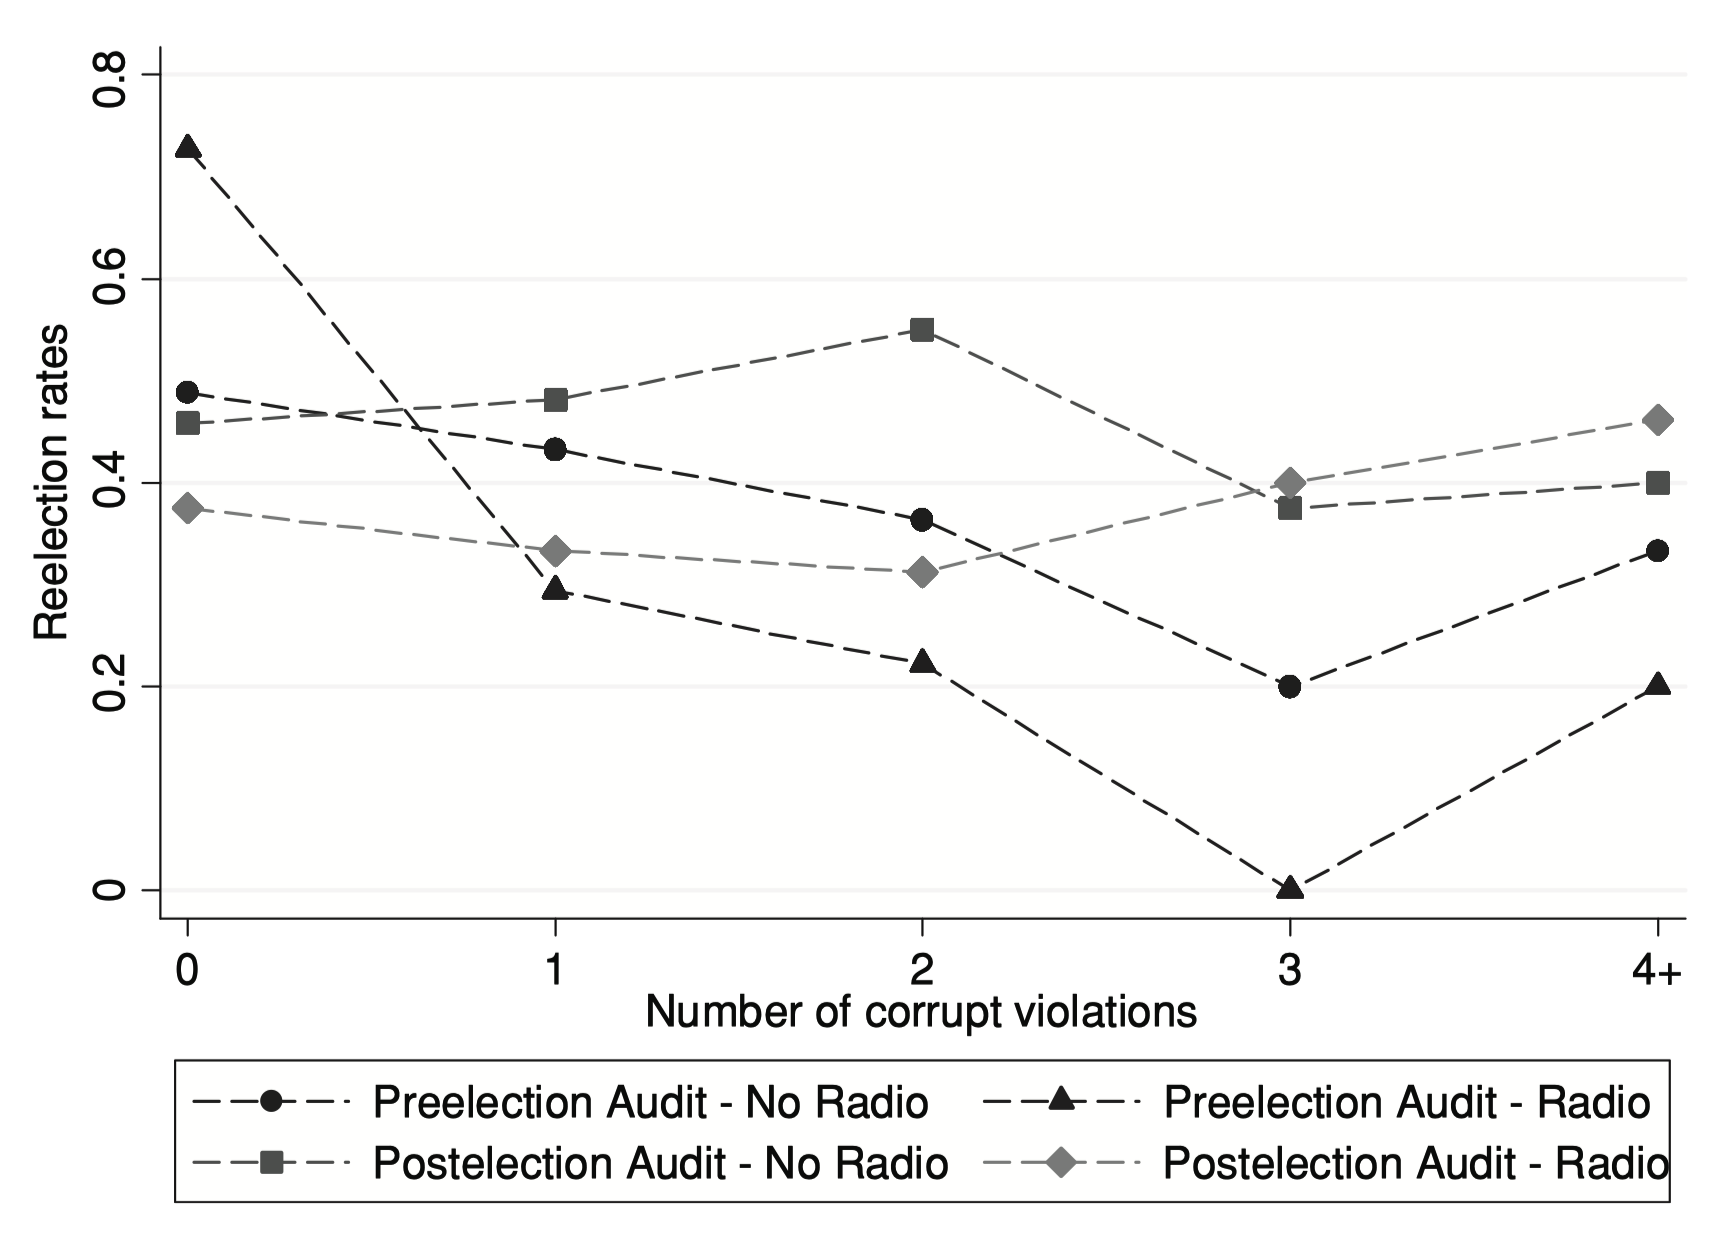
\includegraphics[height = 0.65 \textheight]{images/fig4.png}
            \end{figure}
        \end{column}

        \begin{column}{0.5\textwidth}

            \only<1->{
                \scriptsize
                \begin{align*}
                E_{ms} = & \alpha + \beta_0C_{ms} + \beta_1 A_{ms} + \textcolor{orange}{\beta_2} M_{ms} \\
                & + \textcolor{orange}{\beta_3} \left(A_{ms}\times M_{ms}\right) + \textcolor{orange}{\beta_5}\left(M_{ms}\times C_{ms}\right)\\
                & + \beta_4\left(A_{ms}\times C_{ms}\right) \\
                & + \textcolor{orange}{\beta_6} \left( A_{ms}\times C_{ms}\times M_{ms} \right) + X_{ms}\gamma+\nu_s +\epsilon_{ms}
                \end{align*}
            }

            \only<2->{
                \begin{itemize}
                    \item<2-> \textcolor{orange}{$\beta_6<0$}
                    \item<3-> \textcolor{orange}{$\beta_5>0$}, $\beta_4=0$, \textcolor{orange}{$\beta_3>0$}
                    \item<4-> \textcolor{orange}{$\beta_2<0$}, $\beta_1=0$, $\beta_0=0$ 
                \end{itemize}
            }

        
        \end{column}

    \end{columns}

\end{frame}

    %\section{Discussion}
    
    \frame{\sectionpage}
    
    \begin{frame}{\textit{Robustness check:} Concerns addressed}

        \begin{enumerate}
            \item<2-> Audit process manipulation
            \only<2->{
                \begin{itemize}
                    \item<3-> Control for \textbf{\color{orange}corrupted auditors}: state fixed effects {\scriptsize (Q: standard error)}
                    \item<4-> Control for mayors' \textbf{\color{orange}political power}: party information {\scriptsize (Table V Column 1-4)}
                    \item<5-> Control for mayors' idiosyncratic \textbf{\color{orange}incentives to bribe}: narrow win for 1st term in 2000 {\scriptsize (Table V Column 2-4)}
                \end{itemize}
            }
            \item<6-> Dynamic: early audit treatments induce a learning effect
            \begin{itemize}
                \item<7-> Re-estimate on sub-samples of \textbf{\color{orange}different time windows} {\scriptsize (Table V Column 5-6)}
            \end{itemize}

            \item<8-> Placebo test: the audit treatment is not correlated with 2000 election results.
            
        \end{enumerate}
    
    \end{frame}

    \begin{frame}{\textit{Robustness check:} Concerns addressed}

        \begin{enumerate}
            \item<1-> Media availability: Is it just a proxy?
            \begin{itemize}
                \item<2-> \textbf{\color{orange}eduation level}: audit information is better received/interpreted, educated citizens are more politically engaged
                \item<3-> \textbf{\color{orange}polulation size}: political scandals travel faster in the bigger crowd
                \item<4-> \textbf{\color{orange}economic diversity}: audit information is not so important in municipalities with high income inequality
            \end{itemize}

            \only<5->{Control for these factors, the effect of media presence is stable and significant.}

            \item<6-> Different measures of electoral outcomes and media presence
        \end{enumerate}
    
    \end{frame}
    
    \begin{frame}{What are other concerns?}
        \begin{enumerate}
            \item<1-> Voters' behavior (partially addressed):
            \only<2->{
                \begin{itemize}
                    \item[-] Heterogeneity in beliefs and the formation of beliefs
                    \item[-] How voters think about and react to corruption
                    \item[-] Asymmetry of punishment and reward after the \textit{shock}
                \end{itemize}
            }
            \item<3-> Spillover effects (partially addressed):
            \only<4->{
                \begin{itemize}
                    \item[-] Between politicians
                    \item[-] Between municipalities/individual voters
                    \item[-] Between auditor teams
                \end{itemize}
            }
            \item<5-> Long term effect for politicians seeking for higher positions
            \item<6-> Magnitude of corruption 
            \item<7-> Next-step consequences (reduction of corruption, studied in \citet{avis2018government})
        \end{enumerate}

    \end{frame}

    \begin{frame}{Final Comments}
        \begin{columns}[T]

            \begin{column}{0.4\textwidth}
                \begin{block}{\small \textbf{What I like...}}
                \footnotesize
                    \only<1->{\begin{itemize}
                        \item<1-> empirical completeness
                        \item<2-> a \textit{clean} study
                        \item<3-> good attempt on revealing the mechanism behind
                    \end{itemize}}
                \end{block}
            \end{column}
            
            \begin{column}{0.4\textwidth}
            
            \only<1->{
            \begin{block}{\small \textbf{What I don't like}}
            \footnotesize
               \only<1->{\begin{itemize}
                   \item<4-> \textit{too} reduced-form
                   \item<5-> \textit{so} much anecdotal evidence that it becomes un-informative
                   \item<6-> TYPOS, in tables :(
               \end{itemize}}
            \end{block}
            }
            
            \end{column}
            \end{columns}
    \end{frame}

\section*{References}
\begin{frame}[allowframebreaks]{References}
    \printbibliography[heading=none]
\end{frame}
    
\part{}
    \begin{frame}[plain,c]
    \begin{center}
       \Huge
        \textcolor{mygreen}{Thank you!} 
        
    \end{center}
    \end{frame}
\end{document}
